%-----------------------------------------------------------------------
%
%   UFRJ  - Universidade Federal do Rio de Janeiro
%   COPPE - Coordena��o dos Programas de P�s-gradua��o em Engenharia
%   PEE   - Programa de Engenharia El�trica
%
%   COE-835  Controle adaptativo
%
%   Relat�rio da simula��o
%                                                         Ramon R. Costa
%                                                         05/out/09, Rio
%-----------------------------------------------------------------------
\documentclass[11pt,a4paper]{article}
\usepackage[latin1]{inputenc} %pacote para utilizar palavras acentuadas
\usepackage{amsmath,amssymb}  %pacotes do AMS
\usepackage{latexsym}         %pacote para incluir s�mbolos (ex.\Box)
\usepackage{fancybox,fancyhdr}%pacote com frescuras
\usepackage{graphicx}         %pacote para incluir figuras tipo eps
\usepackage[portuguese]{babel}
\usepackage{xcolor}
\usepackage{float} 
\usepackage{epstopdf}
\usepackage[inline]{enumitem}
\usepackage[a4paper]{hyperref}% Make sure it comes last of your loaded packages
\hypersetup{
  verbose,
  plainpages=false,
  bookmarks=true,
  colorlinks=true,
  linkcolor=blue
}

%Matlab code in latex 
\usepackage[final]{listings}
\usepackage{color} %red, green, blue, yellow, cyan, magenta, black, white
\definecolor{mygreen}{RGB}{28,172,0}
\definecolor{mylilas}{RGB}{170,55,241}
\lstdefinestyle{myMatlab}
{
language=matlab,frame=single, basicstyle=\small\ttfamily,breaklines=true,%
morekeywords={matlab2tikz}, keywordstyle=\color{blue}, morekeywords=[2]{1}, keywordstyle=[2]{\color{black}}, commentstyle=\color{mygreen}, stringstyle=\color{mylilas}, identifierstyle=\color{black}, showstringspaces=false,%without this there will be a symbol in the places where there is a space
numbers=left, numberstyle={\scriptsize \color{black}},% size of the numbers
numbersep=9pt, % this defines how far the numbers are from the text
% emph=[1]{for,end,break},emphstyle=[1]\color{red}, %some words to emphasise
% emph=[2]{word1,word2}, emphstyle=[2]{style},
}
     
%----------------------------------------------------------------------
%
%   Macros utilizados no LATEX
%                                                       Ramon R. Costa
%                                                       13/out/17, Rio
%----------------------------------------------------------------------
\newcount\m
\newcount\n

\def\twodigits#1{\ifnum #1<10 0\fi \number#1}

\def\hours{\n=\time \divide\n 60
    \m=-\n \multiply\m 60 \advance\m \time
    \twodigits\n:\twodigits\m}

\def\hora{\hours}

\def\fim{
  \medskip
  \begin{center}
    \rule[1mm]{30mm}{0.14mm}$\diamond$\rule[1mm]{30mm}{0.14mm}
  \end{center}
}

%----------------------------------------------------------------------
% A4 paper size & margins
\setlength {\textheight}    {25cm}%
\setlength {\textwidth}     {17.5cm}%
\setlength {\parindent}     {0mm}%
\setlength {\parskip}       {1mm}%
\setlength {\topmargin}     {-14mm}%
\setlength {\oddsidemargin} {-6mm}%
\setlength {\evensidemargin}{-6mm}%
\setlength {\columnsep}     {6mm}%

%----------------------------------------------------------------------
\def\codigo{COE-835}
\def\disciplina{Controle adaptativo}
\def\periodo{3o. período/2017}
\def\professor{Ramon}

\newcommand{\BOX}[1]{
  \framebox{{\color{magenta}\rule[-3mm]{1mm}{9mm}} ~~$\displaystyle
  \begin{aligned} #1 \end{aligned}$~~}\pagestyle{plain}
}

\newcommand{\RED}[1]{\colorbox{white}{\textcolor{red}{#1}}}
%\newcommand{\WoR}[1]{\colorbox{red}{\textcolor{white}{#1}}}
\newcommand{\BLU}[1]{\colorbox{white}{\textcolor{blue}{#1}}}
\newcommand{\GRE}[1]{\colorbox{green}{\textcolor{black}{#1}}}
\newcommand{\HI}[1]{\colorbox{yellow}{\textcolor{black}{#1}}}  %% Highlithed text

\newcommand{\estrela}[1]{
  \def\TXT{\RED{$\bigstar$ }}
  \hspace*{5mm}\TXT \hfill
  \parbox[t]{ \textwidth - \widthof{\TXT} - 5mm}{#1}
  \par
}

\def\Ltwo{\mbox{${\mathcal L}_2$}}
\def\Linf{\mbox{${\mathcal L}_\infty$}}

\newcommand{\sign}{\mbox{sign}}

\newcommand{\equacao}[2]{
  \makebox[50mm][l]{#1 \dotfill}: \quad %\parbox[t]{10cm}
	{\begin{equation*} \displaystyle
  \begin{aligned}
    #2
  \end{aligned} \end{equation*}} \\
}

\newcommand{\sref}[1]{Section~\ref{#1}}
\newcommand{\fref}[1]{Fig.~\ref{#1}}
\newcommand{\tref}[1]{Table~\ref{#1}}
\newcommand{\thref}[1]{Theorem~\ref{#1}}
\newcommand{\aref}[1]{Assumption~\ref{#1}}
\newcommand{\norm}[1]{\left\lVert#1\right\rVert}
%\renewcommand{\qedsymbol}{}
\newcommand{\rev}[1]{{\color{red}#1}}
\newcommand{\mat}[1]{\begin{bmatrix}#1\end{bmatrix}}

\newtheorem{remark}{Remark}
\newtheorem{lemma}{Lema}

%----------------------------------------------------------------------


%Set normal paragraph spacing
\setlength\parindent{24pt}

\begin{document}
%---------------------------------------------------------------------
\pagestyle{fancy}%
\renewcommand{\headrulewidth}  {0.4pt}%
\renewcommand{\footrulewidth}  {0.4pt}%
\lhead{\bfseries{Relat�rio do Trabalho 9}}%
\chead{}%
\rhead{\bfseries\thepage}%
\lfoot{}%
\cfoot{}%
\rfoot{[\hours] \quad \today}%
%---------------------------------------------------------------------
\begin{center}
  \huge{COE-835  Controle  adaptativo}  \\[20mm]

  \Large{Trabalho 9} \\[20mm]
\end{center}

\textbf{Grupo:} \quad \parbox[t]{10cm}{
Guilherme Pires Sales de Carvalho \\[2mm]
Matheus Ferreira dos Reis \\[2mm]
Renan Salles de Freitas \\[10mm]
}

\textbf{Algoritmo:} \quad \HI{Direct Adaptive Backstepping Control (Reduced
Order Observer)}\\[2mm]

\bigskip%
\textbf{Caso}: \quad \parbox[t]{10cm}{
  $n = 2$ \quad (ordem da planta) \\[2mm]
  $n^* = 2$ \quad (grau relativo) \\[2mm]
  $n_p = 3$ \quad (\# de par�metros) \\[15mm]
}

%---------------------------------------------------------------------
\tableofcontents
\newpage
%---------------------------------------------------------------------
%---------------------------------------------------------------------
\section{Backstepping - Formula��o te�rica sem observador}

Backstepping � um m�todo recursivo de controle adaptativo baseado em Lyapunov e
proposto no come�o da d�cada de 90. A ideia � projetar um controle recursivo
considerando algumas das vari�veis de estado como ``controle virtuais'' e
implementar para elas leis de controle intermedi�rias. Com esta t�cnica �
poss�vel resolver problemas de estabilidade e rastreamento. Neste trabalho,
desenvolveremos a fundamenta��o te�rica para o caso de um sistema de
segunda ordem com par�metros desconhecidos:
%
\begin{align}
\dot{x}_1 &= x_2 + \phi_1^\intercal(x_1) \, \theta\\
\nonumber \dot{x}_2 &= k_p\,u + \phi_2^\intercal(x_1,x_2)\,\theta\\
\nonumber y &= x_1\,,
\label{eq:planta}
\end{align}
%
onde $\theta$ � o vetor de par�metros desconhecidos e $k_p$ � o ganho de
alta frequ�ncia, tamb�m desconhecido. As n�o linearidades do sistema s�o
representadas pela vari�vel $\phi$. Para o desenvolvimento do algoritmo,
assume-se:
%
\begin{itemize}
  \item o sinal de $k_p$ � conhecido;
  \item o sinal de refer�ncia $y_r$ e suas derivadas s�o cont�nuas e limitadas.
\end{itemize}

Introduzem-se as vari�veis $\textbf{z}$ (mudan�a de coordenadas):
%
\begin{align}
z_1 &= y - y_r \\
\nonumber z_2 &= x_2 - \alpha_1 - \dot{y}_r \,,
\end{align}
%
onde $\alpha_1$ � a vari�vel de controle virtual. O primeiro passo para a
elabora��o do m�todo � come�ar pela equa��o \eqref{eq:planta},
considerando $x_2$ como uma vari�vel de controle virtual. A derivada do erro de
rastreamento $z_1$ � dada por:
%
\begin{align}
\dot{z}_1 &= \dot{x}_1 - \dot{y}_r \\
\nonumber &= z_2 + \alpha_1 + \phi_1^\intercal\,\theta
\end{align}

Podemos projetar a primeira fun��o estabilizante $\alpha_1$ como:
%
\begin{equation}
\alpha_1 = -c_1z_1 - \phi_1^\intercal\,\hat{\theta},
\end{equation}
%
onde $c_1$ � uma constante positiva e $\hat{\theta}$ � uma estimativa de
$\theta$. Consideremos a fun��o de Lyapunov:
%
\begin{equation}
V_1 = \frac{1}{2}z_1^2 +
\frac{1}{2}\tilde{\theta}^\intercal\,\Gamma^{-1}\,\tilde{\theta},
\end{equation}
%
onde $\Gamma$ � uma matriz positiva definida e
$\tilde{\theta}=\theta-\hat{\theta}$. Derivando a fun��o de Lyapunov, temos:
%
\begin{align}
\dot{V}_1 &= z_1\dot{z}_1 -
\tilde{\theta}^\intercal\,\Gamma^{-1}\,\dot{\hat{\theta}}\\
\nonumber &=
z_1(z_2+\alpha_1+\phi_1^\intercal
\, \hat{\theta})-\tilde{\theta}^\intercal(\Gamma^{-1} \,
\dot{\hat{\theta}}-\phi_1z_1)\\
\nonumber &= -c_1z_1^2+\tilde{\theta}^\intercal(\tau_1-\Gamma^{-1} \,
\dot{\hat{\theta}}) + z_1z_2\\
\tau_1 &= \phi_1z_1
\end{align}

Observe que se escolhermos a varia��o dos par�metros como
$\dot{\hat{\theta}}=\Gamma\,\tau_1$ anulamos um dos termos, mas ainda falta
considerar a din�mica de $z_2$ na equa��o de Lyapunov e resta ainda o termo $z_1 z_2$. Ent�o, devemos deixar a escolha da lei de adapta��o de $\theta$ em aberto.
%
Agora, derivando $z_2$, temos:
 %
\begin{align}
\dot{z}_2 &= k_pu + \phi_2^\intercal \, \theta - \dot{\alpha_1}-\ddot{y}_r \\
\nonumber &= k_pu + \phi_2^\intercal \, \theta -
\frac{\partial\alpha_1}{\partial x_1}(x_2 + \phi_1^\intercal \, \theta) -
\frac{\partial\alpha_1}{\partial \hat{\theta}}\dot{\hat{\theta}} -
\frac{\partial\alpha_1}{\partial y_r}\dot{y}_r - \ddot{y}_r
\end{align}

Escolhemos a fun��o Lyapunov:
%
\begin{align}
V = V_1 + \frac{1}{2}z_2^2 + \frac{|k_p|}{2\gamma}\tilde{p}^2, 
\end{align}

onde $\tilde{p}=p-\hat{p}$ e $\hat{p}$ � estimativa de $p = \frac{1}{k_p}$, e
$\gamma > 0$. Derivando a fun��o Lyapunov, obtemos:

\begin{align}
\dot{V} =& -c_1z_1^2 + z_1z_2 +
\tilde{\theta}^\intercal(\tau_1-\Gamma^{-1}\dot{\hat{\theta}}) + z_2\dot{z}_2 +
\frac{|k_p|}{\gamma}\tilde{p}\dot{\tilde{p}} \notag\\
\nonumber =& -c_1z_1^2 + z_1z_2 +
\tilde{\theta}^\intercal(\tau_1-\Gamma^{-1}\dot{\hat{\theta}}) + z_2\left( k_pu
+ \phi_2^\intercal \, \theta - \frac{\partial\alpha_1}{\partial x_1}(x_2 + \phi_1^\intercal \, \theta) -
\frac{\partial\alpha_1}{\partial \hat{\theta}}\dot{\hat{\theta}} -
\frac{\partial\alpha_1}{\partial y_r}\dot{y}_r - \ddot{y}_r \right) +
\frac{|k_p|}{\gamma}\tilde{p}\dot{\tilde{p}} \\
%\theta =& \tilde{\theta} + \hat{\theta} \notag\\
=& -c_1z_1^2 + z_1z_2 +
\tilde{\theta}^\intercal(\tau_1-\Gamma^{-1}\dot{\hat{\theta}}) + z_2\left( k_pu
+ (\tilde{\theta}^\intercal + \hat{\theta}^\intercal)(\phi_2 -
\frac{\partial\alpha_1}{\partial x_1}\phi_1) - \frac{\partial\alpha_1}{\partial
x_1}x_2 - \frac{\partial\alpha_1}{\partial 
\hat{\theta}}\dot{\hat{\theta}} + \cdots \right. \notag\\
&\left.  \cdots - \frac{\partial\alpha_1}{\partial y_r}\dot{y}_r - \ddot{y}_r \right) +
\frac{|k_p|}{\gamma}\tilde{p}\dot{\tilde{p}} \notag
\end{align}
%
\begin{align}
\tau_2 =& \,\, \tau_1 + \left(\phi_2 - \frac{\partial\alpha_1}{\partial x_1}\phi_1
\right)z_2  \notag \\
\dot{V} =& -c_1z_1^2 + z_1z_2 +
\tilde{\theta}^\intercal(\tau_2-\Gamma^{-1}\dot{\hat{\theta}}) + z_2\left( k_pu
+ \hat{\theta}^\intercal(\phi_2 -
\frac{\partial\alpha_1}{\partial x_1}\phi_1) - \frac{\partial\alpha_1}{\partial
x_1}x_2 %\right. \notag\\ &\phantom{{}=1} \left. 
- \frac{\partial\alpha_1}{\partial 
\hat{\theta}}\dot{\hat{\theta}} - \frac{\partial\alpha_1}{\partial y_r}\dot{y}_r - \ddot{y}_r \right) +
\frac{|k_p|}{\gamma}\tilde{p}\dot{\tilde{p}} \notag \\
\label{eq:dotV} 
\end{align}

Escolhemos a lei de controle:
%
\begin{align}
u &= \hat{p}\bar{u}\\
\bar{u} &= \alpha_2 + \ddot{y}_r
\end{align}

Note que:
%
\begin{equation}
 k_pu = k_p\hat{p}\bar{u}=\bar{u} - k_p\tilde{p}\bar{u}
 \label{eq:kpu}
\end{equation}

Substituindo a eq.\eqref{eq:kpu} em eq.\eqref{eq:dotV}, temos:
%
\begin{align}
\dot{V} =& -c_1z_1^2 + z_1z_2 +
\tilde{\theta}^\intercal(\tau_2-\Gamma^{-1}\dot{\hat{\theta}}) + z_2\left( \bar{u} - k_p\tilde{p}\bar{u}
+ \hat{\theta}^\intercal(\phi_2 -
\frac{\partial\alpha_1}{\partial x_1}\phi_1) - \frac{\partial\alpha_1}{\partial
x_1}x_2 + \cdots \right. \notag\\
& \left. \cdots - \frac{\partial\alpha_1}{\partial 
\hat{\theta}}\dot{\hat{\theta}} - \frac{\partial\alpha_1}{\partial y_r}\dot{y}_r - \ddot{y}_r \right) +
\frac{|k_p|}{\gamma}\tilde{p}\dot{\tilde{p}} \notag \\
% =& -c_1z_1^2 + z_1z_2 +
% \tilde{\theta}^\intercal(\tau_2-\Gamma^{-1}\dot{\hat{\theta}}) + z_2\left( \bar{u} 
% + \hat{\theta}^\intercal(\phi_2 -
% \frac{\partial\alpha_1}{\partial x_1}\phi_1) - \frac{\partial\alpha_1}{\partial
% x_1}x_2 + \cdots \right. \notag\\
% & \cdots \left. - \frac{\partial\alpha_1}{\partial 
% \hat{\theta}}\dot{\hat{\theta}} - \frac{\partial\alpha_1}{\partial y_r}\dot{y}_r - \ddot{y}_r \right) +
% \frac{|k_p|}{\gamma}\tilde{p}\,\left(\dot{\tilde{p}}-\text{sign}(k_p)\gamma\bar{u}z_2
% \right)
% \\
\nonumber =& -c_1z_1^2 + z_1z_2 +
\tilde{\theta}^\intercal(\tau_2-\Gamma^{-1}\dot{\hat{\theta}}) + z_2\left( \alpha_2
+ \hat{\theta}^\intercal(\phi_2 -
\frac{\partial\alpha_1}{\partial x_1}\phi_1) - \frac{\partial\alpha_1}{\partial
x_1}x_2 + \cdots \right. \notag\\ & \left. \cdots
- \frac{\partial\alpha_1}{\partial 
\hat{\theta}}\dot{\hat{\theta}} - \frac{\partial\alpha_1}{\partial y_r}\dot{y}_r
\right) - \frac{|k_p|}{\gamma}\tilde{p} \,
\left(\dot{\hat{p}}+\text{sign}(k_p)\gamma\bar{u}z_2\right)
\label{eq:dotV2}
\end{align}

Escolhemos $\alpha_2$ como:
%
\begin{equation}
\alpha_2 = -c_2z_2 - z_1 - \hat{\theta}^\intercal(\phi_2 -
\frac{\partial\alpha_1}{\partial x_1}\phi_1) + \frac{\partial\alpha_1}{\partial
x_1}x_2 + \frac{\partial\alpha_1}{\partial \hat{\theta}}\dot{\hat{\theta}} +
\frac{\partial\alpha_1}{\partial y_r} \dot{y}_r
\label{eq:alpha2}
\end{equation}

Substituindo a eq.\eqref{eq:alpha2} em eq.\eqref{eq:dotV2}, obtemos:
%
\begin{align}
\dot{V} &= -c_1z_1^2 -c_2z_2^2 +
\tilde{\theta}^\intercal(\tau_2-\Gamma^{-1}\dot{\hat{\theta}}) -
\frac{|k_p|}{\gamma}\tilde{p} \,
\left(\dot{\hat{p}}+\text{sign}(k_p)\gamma\bar{u}z_2\right)
\end{align}

A lei de atualiza��o dos par�metros �, portanto, escolhida como:
%
\begin{align}
\dot{\hat{p}} &= -\gamma \, \text{sign}(k_p) \, \bar{u} \, z_2 \\
\dot{\hat{\theta}} &= \Gamma\tau_2 
\end{align}

\section{Backstepping - Formula��o te�rica com observador}

No caso pr�tico, os estados da planta nem sempre est�o dispon�veis, de modo que deve-se utilizar um observador para estimar esses estados. Neste trabalho, consideramos o seguinte sistema:
%
\begin{align}
\dot{x}_1 &= x_2 - a_1y \label{eq:planta2}\\
\nonumber \dot{x}_2 &= k_p\,u - a_0y \,,
\end{align}
%
onde o vetor de par�metros $\theta^{\intercal} = \mat{a_1 \,\, a_0 \,\, k_p}$ � desconhecido. Para esta formula��o apenas a sa�da do sistema $y$ est� dispon�vel, $x_2$ n�o � conhecido e deve ser estimado. Podemos reescrever o sistema \eqref{eq:planta2}:
%
\begin{gather}
\dot{x} = Ax + F(y,u)^\intercal\theta \\ \nonumber
A = \mat{0 & 1 \\ 0 & 0} ,\enskip
%
F(y,u)^\intercal = \mat{B(u) & \Phi(y)} ,\enskip
%
\Phi(y) = \mat{-y & 0 \\ 0 & -y} ,\enskip
%
B(u) = \mat{0 \\ u} ,\enskip
%
\theta = \mat{k_p \\ a_1 \\ a_0} ,\enskip
%
y = e_1^\intercal x ,
\end{gather}
%
em que $e_1^\intercal = \mat{1 & 0}$.
%
Para estimar os estados, utilizamos os filtros abaixo:
%
\begin{align}
\label{eq:filtros2}
\dot{\xi} &= A_0\xi + ky \\
\nonumber \dot{\Omega}^\intercal &= A_0\Omega^\intercal + F^\intercal
\end{align}
%
\begin{equation*}
k^\intercal = \mat{k_1 & k_2} \qquad A_0 = A - ke_1^\intercal =  \mat{-k_1 & 1\\-k_2 & 0}
\end{equation*}

Os valores de $k$ devem ser escolhidos de forma que $A_0$ seja Hurwitz. E, dessa
forma, o estado estimado pode ser escrito como:
%
\begin{align}\label{eq:estimador}
\hat{x} = \xi + \Omega^\intercal\theta
\end{align}

Derivando a equa��o \eqref{eq:estimador} e substituindo as equa��es dos
filtros \eqref{eq:filtros2}, verifica-se que a din�mica do estimador � igual �
din�mica da planta \eqref{eq:planta2}.

Por�m, $\Omega$ � uma matriz e opta-se pela redu��o das ordens dos
filtros. Observe que $\Omega^\intercal = \left[v_0 \quad | \quad \Xi\right]$ e,
pela equa��o ~\eqref{eq:filtros2}, temos que:
%
\begin{align}
\dot{v}_0 &= A_0v_0 + e_2u \\
\dot{\Xi} &= A_0\Xi - Iy
\end{align}

Introduzem-se dois novos filtros, para substituir os filtros da
equa��o~\eqref{eq:filtros2}:
%
\begin{align}
\dot{\lambda} &= A_0\lambda + e_2u \\
\dot{\eta} &= A_0\eta + e_2y
\end{align}

� f�cil verificar que, para esta planta de segunda ordem sem zeros ($m=0$), $v_0
= \lambda$. Para o caso geral, temos que:
%
\begin{align}
\dot{\lambda} &= A_0\lambda + e_2u \\
v_i &= A_0^i\lambda \quad (i=0,\ldots,m)
\end{align}

� poss�vel demonstrar que:
%
\begin{align}
\Xi &= -\left[A_0\eta \quad \eta\right] \\
\xi &= -A_0^2\eta
\end{align}

Definindo $\omega^\intercal = \mat{v_0 & \left(\Xi_2 - ye_1^\intercal \right)}$, $\bar{\omega}^\intercal = \mat{0 & \left(\Xi_2 - ye_1^\intercal \right)}$ e $\epsilon_2 = x_2 - \hat{x}_2$, reescrevemos a din�mica da sa�da $y$ como:
%
\begin{align}
\dot{y} &= x_2 + \phi^\intercal\theta\\
\nonumber &= k_pv_{0,2} + \xi_2 + \bar{\omega}^\intercal\theta + \epsilon_2
\end{align}

Desta forma, o sistema \eqref{eq:planta2} pode ser representado com os estados do
observador:
%
\begin{align}
\dot{y} &= k_pv_{0,2} + \xi_2 + \bar{\omega}^\intercal\theta + \epsilon_2\\
\dot{v}_{0,2} &= u - k_2v_{0,1} \nonumber
\end{align}

O projeto backstepping agora segue como na se��o anterior. Primeiro, fazemos a
mudan�a de coordenadas em $\mathbf{z}$:
%
\begin{align}
z_1 &= y - y_r \\
\nonumber z_2 &= v_{0,2} - \alpha_{1} - \hat{\rho}\dot{y_r} \,,
\end{align}
%
onde $\hat{\rho}$ � estimativa de $\frac{1}{k_p}$. O controle virtual $\alpha_1$, a
lei de controle $u$ e as leis de adapta��o $\dot{\hat{\theta}}$ e $\dot{\hat{\rho}}$ s�o
obtidas pelo m�todo de Lyapunov. Derivando $z_1$, obtemos:
%
\begin{align}
\dot{z}_1 &= k_p\alpha_1 + \xi_2 + \bar{\omega}^\intercal\theta + \epsilon_2 -
k_p\tilde{\rho}\dot{y}_r+k_pz_2 \\
\alpha_1 &= \hat{\rho}\bar{\alpha}_1\\
\dot{z}_1 &= \bar{\alpha}_1 + \xi_2 + \bar{\omega}^\intercal\theta + \epsilon_2
- k_p(\dot{y}_r + \bar{\alpha}_1)\tilde{\rho} + k_pz_2
\end{align}

E escolhemos a primeira fun��o estabilizante:
%
\begin{align}
\bar{\alpha}_1 = -c_1z_1-d_1z_1-\xi_2-\bar{\omega}^\intercal\hat{\theta}
\end{align}

A din�mica de $z_1$ pode ser reescrita como:
%
\begin{align}
\dot{z}_1 =
-c_1z_1-d_1z_1+\epsilon_2+\left[\omega-\hat{\rho}(\dot{y}_r
+ \bar{\alpha}_1)e_1\right]^\intercal\tilde{\theta} -
k_p(\dot{y}_r+\bar{\alpha}_1)\tilde{\rho} + \hat{k}_pz_2
\end{align}

Escolhe-se a fun��o de Lyapunov:
%
\begin{align}
2V_1 = z_1^2 +
\tilde{\theta}^\intercal\Gamma^{-1}\tilde{\theta}+|k_p|\gamma^{-1}\tilde{\rho}^2
+ \frac{1}{2d_1}\epsilon^\intercal P\epsilon
\end{align}

Nessas condi��es, � poss�vel escolher a atualiza��o de $\hat{\rho}$ segundo:
%
\begin{align}
\dot{\hat{\rho}} &= -\gamma z_1 \text{sign}(k_p)(\dot{y}_r + \bar{\alpha}_1)
\end{align}

Derivando $z_2$, obtemos:
%
\begin{align}
\dot{z}_2 &= \dot{v}_{0,2} - \hat{\rho}\ddot{y}_r - \dot{\hat{\rho}}\dot{y}_r -
\dot{\alpha}_1 \\
&= u - \hat{\rho}\ddot{y}_r - \beta -
\frac{\partial\alpha_1}{\partial y}(\omega^\intercal\tilde{\theta} + \epsilon_2)
- \frac{\partial\alpha_1}{\partial\hat{\theta}}\dot{\hat{\theta}} \\
\beta &= k_2v_{0,1} + \frac{\partial\alpha_1}{\partial y}(\xi_2 +
\omega^\intercal\hat{\theta}) + \frac{\partial \alpha_1}{\partial \eta}
(A_0\eta + e_2y) + \frac{\partial \alpha_1}{\partial y_r} \dot{y}_r +
(\dot{y}_r + \frac{\partial \alpha_1}{\partial \hat{\rho}})\dot{\hat{\rho}}
\end{align}

Escolhe-se a fun��o de Lyapunov:
%
\begin{align}
V_2 = V_1 + \frac{1}{2}z_2^2 + \frac{1}{4d_2}\epsilon^\intercal P\epsilon
\end{align}

� poss�vel mostrar que a atualiza��o de par�metros e a lei de controle s�o:
%
\begin{align}
\dot{\hat{\rho}} &= -\gamma z_1 \text{sign}(k_p)(\dot{y}_r + \bar{\alpha}_1) \\
\tau_1 &= (\omega - \hat{\rho}(\dot{y}_r + \bar{\alpha}_1)\mat{e_1^\intercal & 0}^\intercal)z_1 \\
\tau_2 &= \tau_1 - z_2 \frac{\partial \alpha_1}{\partial y} \omega \\
\dot{\hat{\theta}} &= \Gamma\tau_2 \\
u &= -c_2z_2 + \beta + \hat{\rho}\ddot{y}_r + \frac{\partial \alpha_1}{\partial
\hat{\theta}} \Gamma \tau_2 - d_2z_2\left( \frac{\partial \alpha_1}{\partial y}\right)^2 - \hat{k}_pz_1
\end{align}

%\section{Implementa��o}

Transcrevemos abaixo a fun��o que computa o Backstepping com observador de ordem reduzida para a forma direta, ou seja, com o vetor $\theta$ contendo os par�metros de controle:

\lstinputlisting[style=myMatlab]{../matlab/backstepping_red_direct.m}
%%---------------------------------------------------------------------
\section{Resultados das simula��es}

Nas simula��es, procuramos avaliar o comportamento do sistema para as seguintes condi��es:
%
\begin{enumerate*}[label=(\roman*)]
\item condi��o inicial $y(0)$;
\item par�metros da planta;
\item sinal de refer�ncia;
\item ganho de adapta��o $\Gamma$.
\end{enumerate*}

Apresentaremos os resultados obtidos atrav�s de simula��es no ambiente \HI{\texttt{Matlab/Simulink}} e os discutiremos na pr�xima se��o.
%
Para todas as simula��es, utilizamos $N = -1$, $c_1 = c_2 = d_1 = d_2 = \gamma = 1$ e condi��es iniciais nulas em todas as din�micas, exceto em $\rho(0) = 1$ e $y(0)$.

\subsection{Simula��o \#1}

Inicialmente, desejamos verificar o comportamento do sistema para varia��es nas
condi��es iniciais.

%
\begin{align*}
  y &= \frac{5}{s^2+2s+1}u\,,  &  y(0) &= \HI{0} \, \textrm{e} \, \HI{10}\,,
  & \Gamma &= 1 \, \textbf{I}_3\,, & y_r &= \textrm{sin}(t) +
  \textrm{sin}(3t) \, .
\end{align*}
%
\begin{figure}[H]
  \centering
  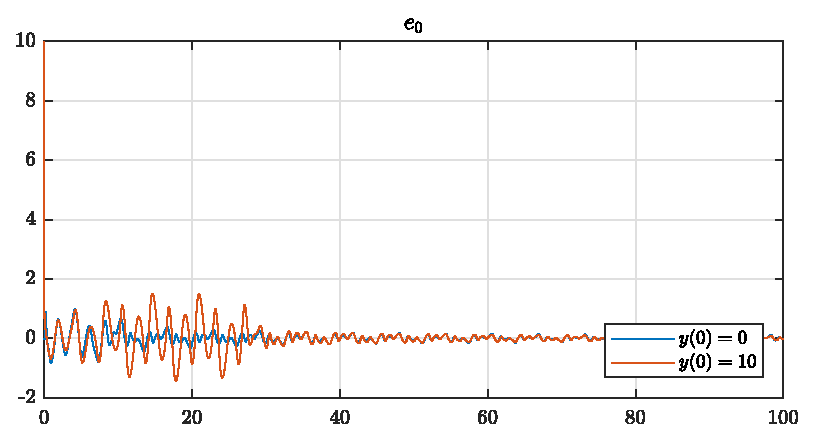
\includegraphics[width=12cm]{figs/e0/y01y02.eps} 
\end{figure}

\begin{figure}[H]
  \centering
  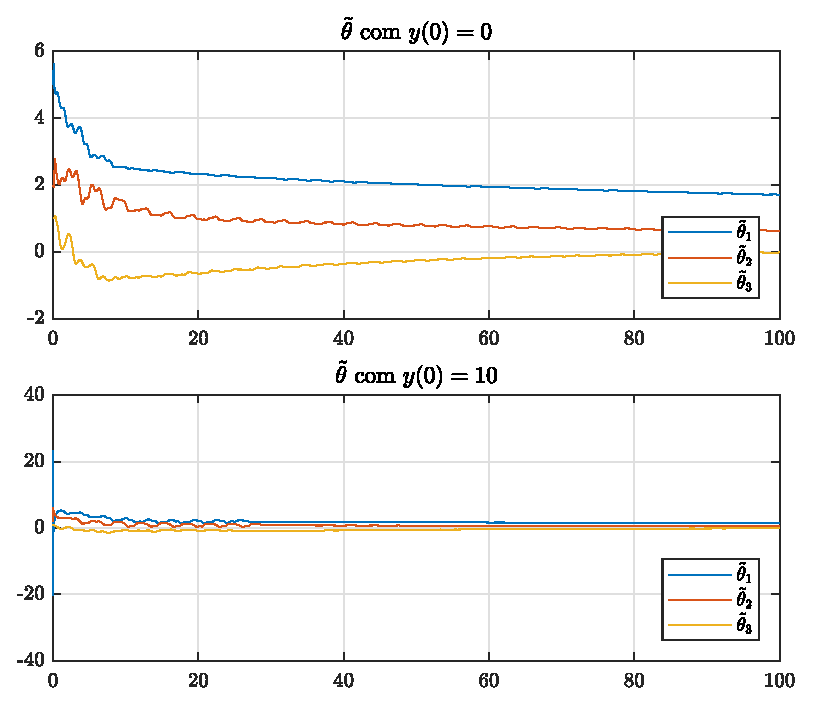
\includegraphics[width=12cm]{figs/tiltheta/y01y02.eps} 
\end{figure}

\begin{figure}[H]
  \centering
  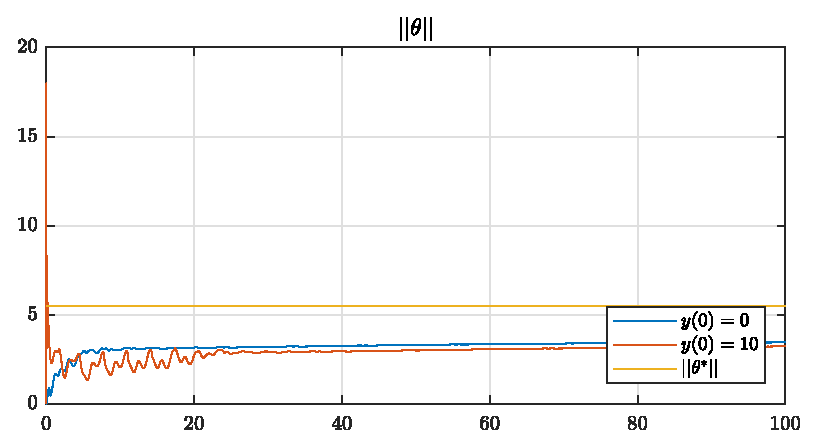
\includegraphics[width=12cm]{figs/modtheta/y01y02.eps} 
\end{figure}

\begin{figure}[H]
  \centering
  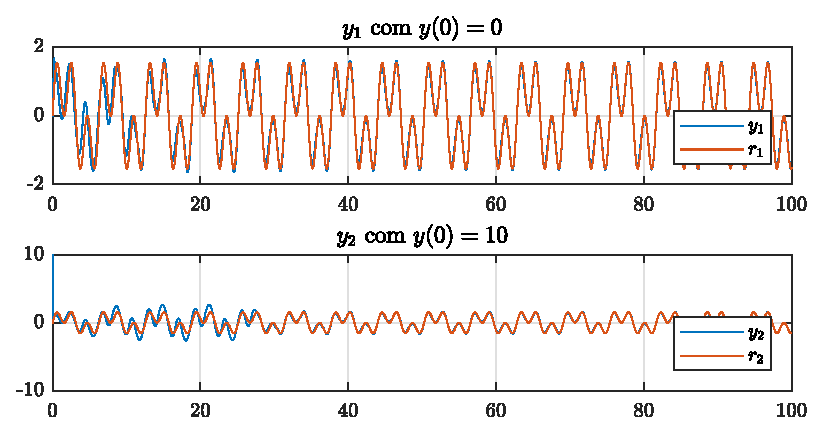
\includegraphics[width=12cm]{figs/y/y01y02.eps} 
\end{figure}

\begin{figure}[H]
  \centering
  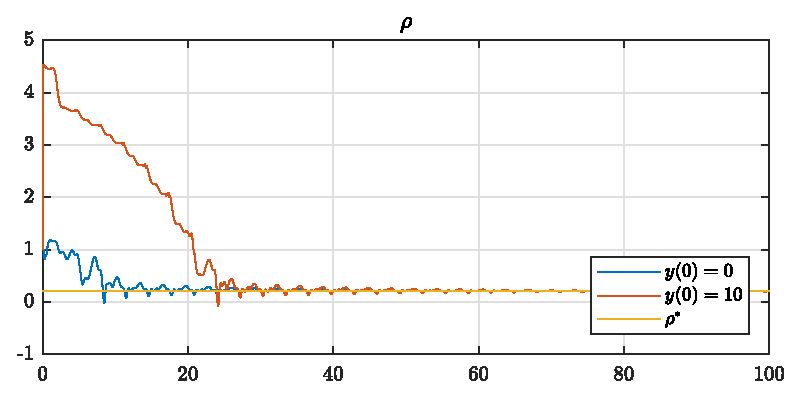
\includegraphics[width=12cm]{figs/rho/y01y02.eps} 
\end{figure}

\subsection{Simula��o \#2}

Verificamos o comportamento do sistema para varia��es nos par�metros da planta.

\begin{align*}
  y &= \HI{$\frac{5}{s^2+2s+1}u$} \,\,\, \textrm{e} \,\,\, \HI{$\frac{2}{s^2-2s+1}u$} \,,  &   y(0) &=  0 \,, & \Gamma &= 1 \,
  \textbf{I}_3\,, & y_r &= \textrm{sin}(t) + \textrm{sin}(3t) \, .
\end{align*}

\begin{figure}[H]
  \centering
  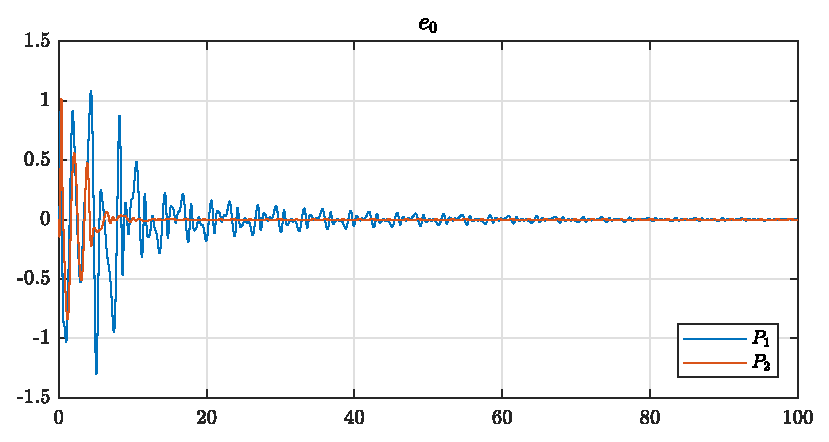
\includegraphics[width=12cm]{figs/e0/P1P2.eps} 
\end{figure}

\begin{figure}[H]
  \centering
  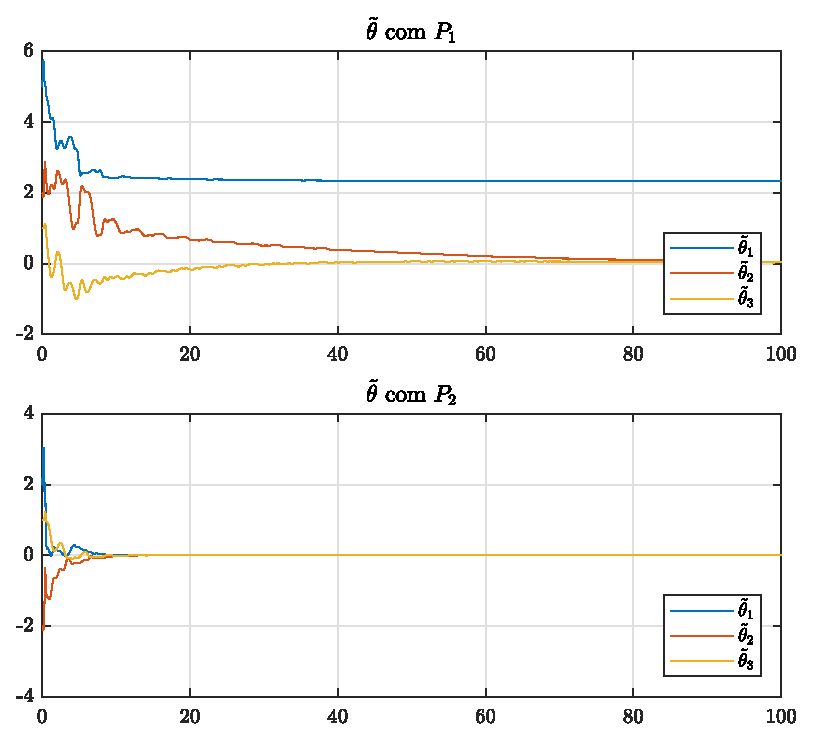
\includegraphics[width=12cm]{figs/tiltheta/P1P2.eps} 
\end{figure}

\begin{figure}[H]
  \centering
  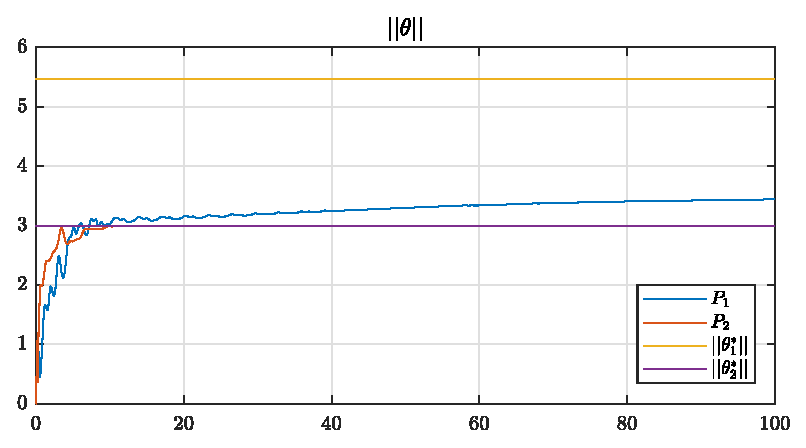
\includegraphics[width=12cm]{figs/modtheta/P1P2.eps} 
\end{figure}

\begin{figure}[H]
  \centering
  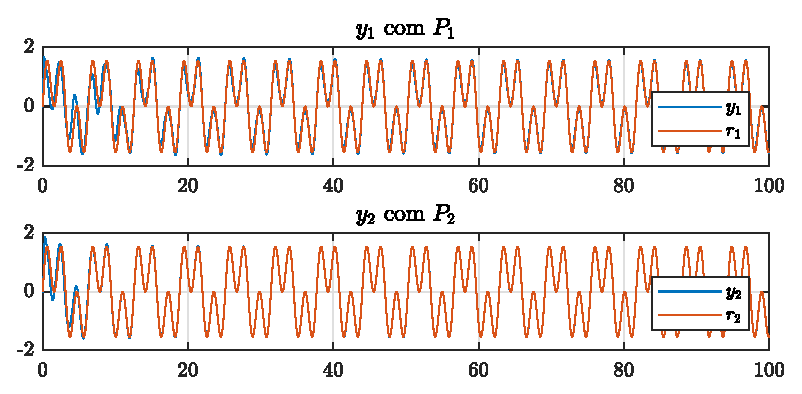
\includegraphics[width=12cm]{figs/y/P1P2.eps} 
\end{figure}

\begin{figure}[H]
  \centering
  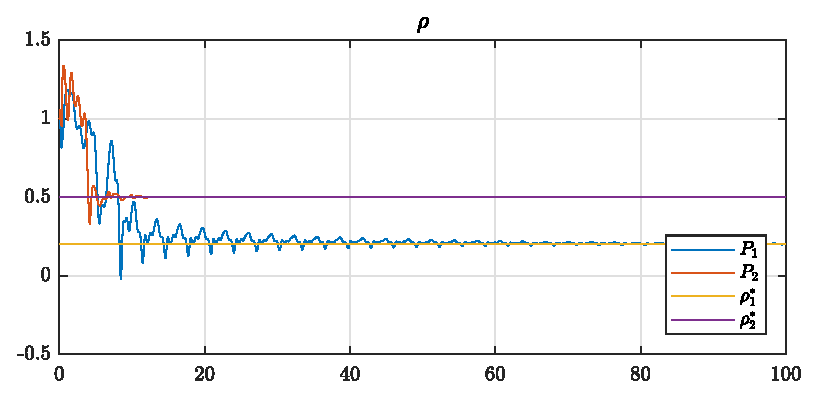
\includegraphics[width=12cm]{figs/rho/P1P2.eps} 
\end{figure}


\subsection{Simula��o \#3}

Verificamos o comportamento do sistema para varia��es no sinal de refer�ncia $y_r(t)$.

\begin{align*}
  y &= \frac{5}{s^2+2s+1}u\,,  & y(0) &=  0 \,, & \Gamma &= 1 \,
  \textbf{I}_3\,, & y_r &= \HI{$\textrm{sin}(t) + \textrm{sin}(3t)$} \,\, \textrm{e} \,\,
  \HI{$\textrm{sin}(t) + \textrm{2sin}(5t)$} \,.
\end{align*}

\begin{figure}[H] 
  \centering
  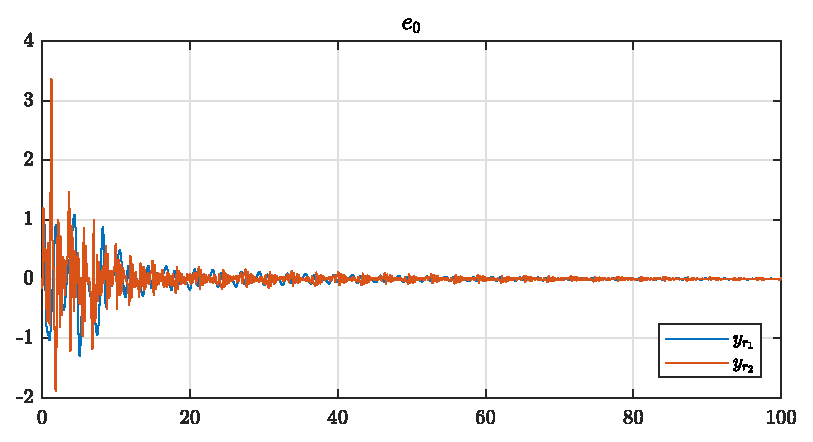
\includegraphics[width=12cm]{figs/e0/yr1yr2.eps} 
\end{figure}

\begin{figure}[H]
  \centering
  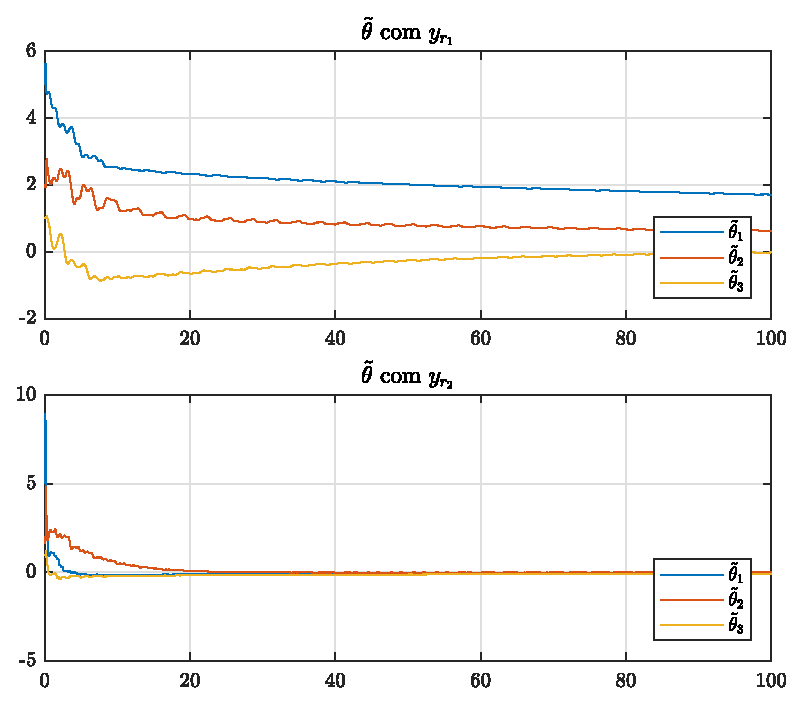
\includegraphics[width=12cm]{figs/tiltheta/yr1yr2.eps} 
\end{figure}

\begin{figure}[H]
  \centering
  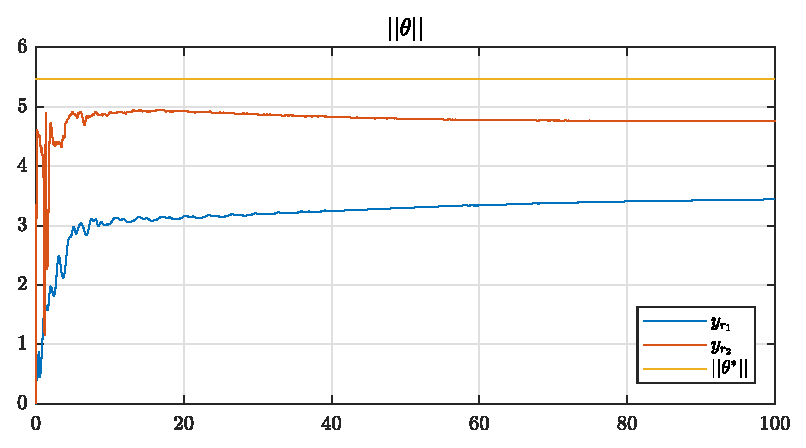
\includegraphics[width=12cm]{figs/modtheta/yr1yr2.eps} 
\end{figure}

\begin{figure}[H]
  \centering
  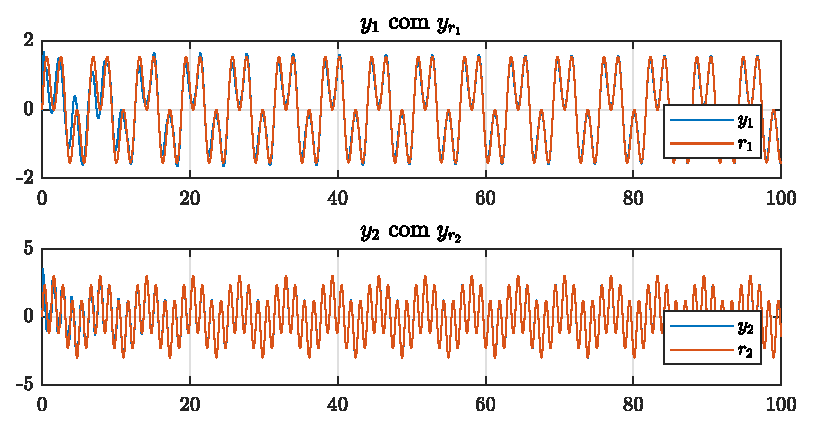
\includegraphics[width=12cm]{figs/y/yr1yr2.eps} 
\end{figure}

\begin{figure}[H]
  \centering
  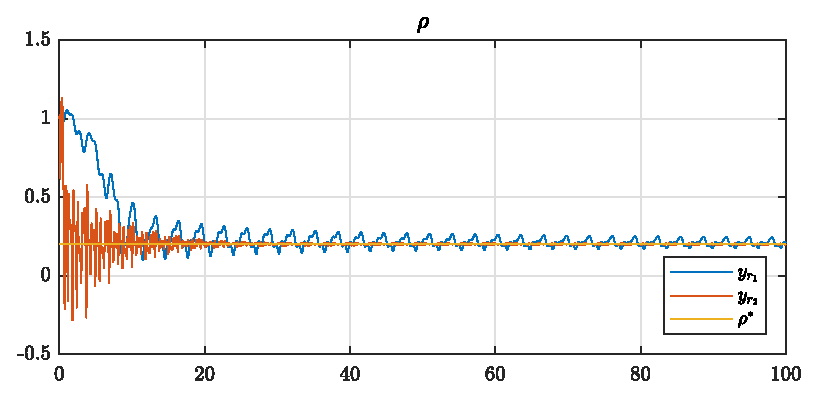
\includegraphics[width=12cm]{figs/rho/yr1yr2.eps} 
\end{figure}

\subsection{Simula��o \#4}

Verificamos o comportamento do sistema para varia��es no ganho de adapta��o $\Gamma$.

\begin{align*}
  y &= \frac{5}{s^2+2s+1}u\,,  & y(0) &=  0 \,, & \Gamma &= \HI{$1 \textbf{I}_3$} \,\, \textrm{e} \,\, \HI{$10 \textbf{I}_3$}\,, & y_r &= \textrm{sin}(t) + \textrm{sin}(3t) \,.
\end{align*}

\begin{figure}[H] 
  \centering
  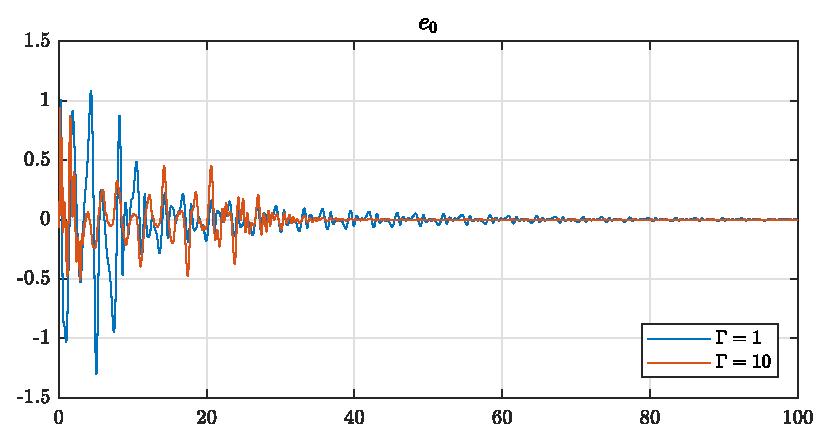
\includegraphics[width=12cm]{figs/e0/Gamma1Gamma10.eps} 
\end{figure}

\begin{figure}[H]
  \centering
  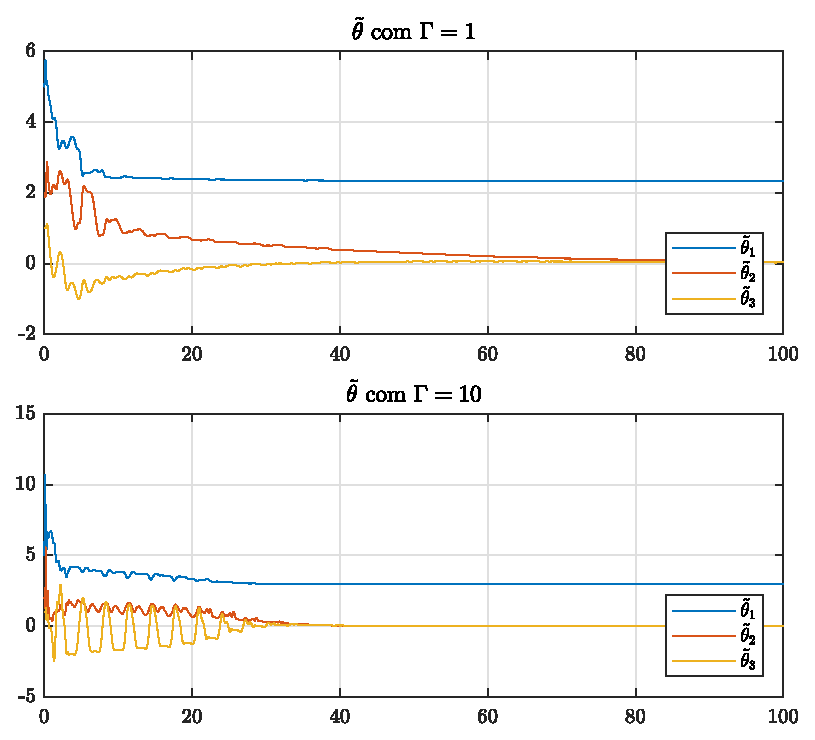
\includegraphics[width=12cm]{figs/tiltheta/Gamma1Gamma10.eps} 
\end{figure}

\begin{figure}[H]
  \centering
  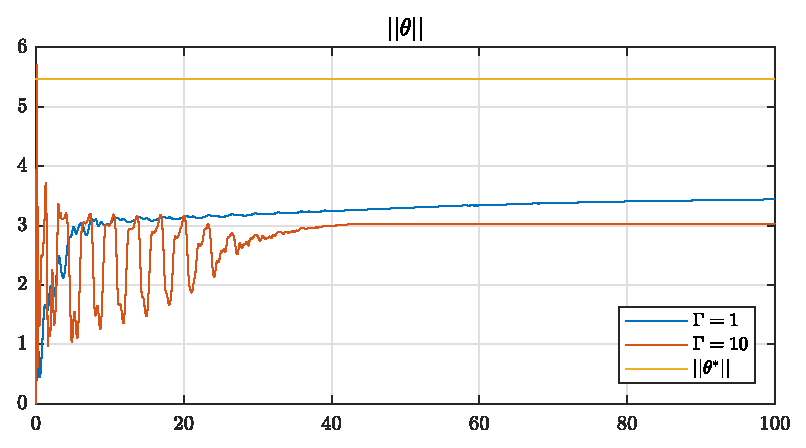
\includegraphics[width=12cm]{figs/modtheta/Gamma1Gamma10.eps} 
\end{figure}

\begin{figure}[H]
  \centering
  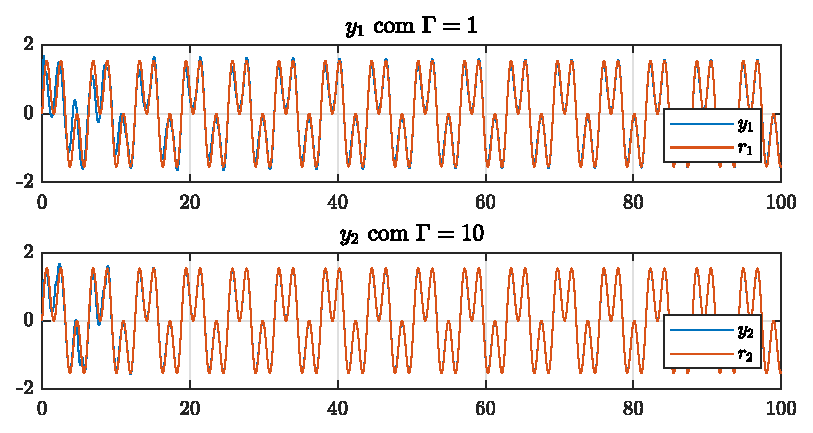
\includegraphics[width=12cm]{figs/y/Gamma1Gamma10.eps} 
\end{figure}

\begin{figure}[H]
  \centering
  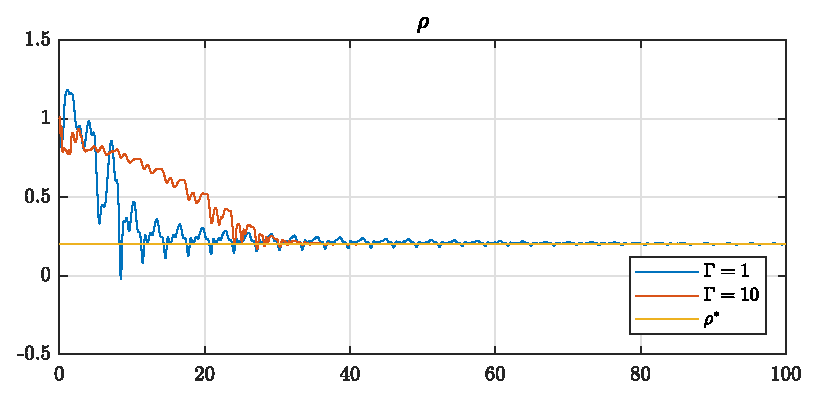
\includegraphics[width=12cm]{figs/rho/Gamma1Gamma10.eps} 
\end{figure}

%%---------------------------------------------------------------------
\section{Discuss�o}

A \textbf{simula��o \#1} mostra o comportamento do sistema para varia��es nas
condi��es iniciais. A rapidez da converg�ncia depende de qu�o pr�ximo os par�metros estimados est�o dos par�metros reais. A simula��o mostrou um comportamento semelhante para ambos os casos. Quando deslocamos o $y(0)$, os sistemas tamb�m
apresentam comportamento semelhante, pois a vari�vel de controle $u$ � alterada
e n�o apresenta satura��o, compensando a condi��o inicial.

A \textbf{simula��o \#2} mostra o comportamento do sistema para varia��es na
planta. Escolhemos plantas inst�veis e est�veis. Podemos observar que, em ambos
os casos, o sinal de controle foi capaz de corrigir o erro, sem muitas
dificuldades. O comportamento dos sistemas � semelhante e para a planta 2, houve at� converg�ncia dos par�metros $\theta$.

Na \textbf{simula��o \#3}, foram testadas duas refer�ncias $y_r$ distintas, que tamb�m podem ser entendidas como a resposta de um modelo de refer�ncia $P_m(s)$ a uma refer�ncia $r(t)$. A altera��o no sinal de refer�ncia mostrou que sinais mais complexos, com frequ�ncias mais altas e maiores amplitudes, demoram um pouco mais para convergir.

Finalmente, a \textbf{simula��o \#4} mostra o comportamento do sistema para varia��es no
ganho de adapta��o $\Gamma$. Podemos verificar converg�ncia mais r�pida quando o
$\Gamma$ � maior, por�m tamb�m observamos maiores oscila��es e picos de erro. 
%---------------------------------------------------------------------
%\bibliographystyle{agsm}
%\bibliography{bib,coe736}

%---------------------------------------------------------------------
\end{document}
